\chapter{Metodolog\'ia y dise\~no de un experimento para inducir ansiedad en cuidadores de personas con demencia}\label{capit:cap3}
\vspace{-2.0325ex}%
\noindent
\rule{\textwidth}{0.5pt}
\vspace{-5.5ex}% 
\newcommand{\pushline}{\Indp}% Indent puede ir o no :p
\section{Introducci\'on}\label{secc:introduction}

Como vimos en el cap\'itulo 2, la mayor\'ia de los estudios logran inducir ansiedad o estr\'es por medio de situaciones controladas dentro del laboratorio. Sin embargo, generar ansiedad en cuidadores informales es mucho mas dif\'icil. El escenario de un laboratorio no coincide con el entorno en el que una persona con demencia se desarrolla por lo que los comportamientos impredecibles no ser\'ian congruentes con dicho ambiente. Adem\'as, exponer a personas sin experiencia ante una persona con demencia que tiene necesidades reales resultar\'ia riesgoso para ambos individuos. Por otra parte, realizar una intervenci\'on totalmente natural a\~nade un grado de dificultad al estudio, resultando en ruido en los datos recolectados (p. ej. la se\~nal de ritmo card\'iaco podr\'ia ser alta no por una situaci\'on de ansiedad, sino por una actividad f\'isica, m\'ultiples distracciones o responsabilidades al mismo tiempo para el cuidador) haciendo d\'ificil de analizarlos.

En este cap\'itulo se explica el uso de una t\'ecnica llamada ``Naturalistic Enactment (NE)'' dentro de un experimento para capturar datos de ansiedad en cuidadores de personas con demencia.


\section{Un experimento para inducir ansiedad en cuidadores informales}\label{secc:experiment}
Se dise\~n\'o una intervenci\'on para inducir ansiedad en cuidadores informales bajo situaciones naturalistas y controladas. Para lograr esto, se utiliz\'o la t\'ecnica de NE. NE fue propuesta originalmente para evaluar tecnolog\'ias m\'edicas ubicuas, donde el tener una validez ambiental e interacc\'on directa del usuario es importante, y donde sin embargo, utilizar pacientes reales puede ser peligroso\citep{Castro11}. NE consiste de el desarrollo de tareas reales (p. ej. la exposici\'on a situaciones y tareas en situaciones naturales) para simular la experiencia del usuario bajo condiciones normales, y por lo tanto encontrar problemas y comportamientos que pudieran de otra manera haber sido dif\'iciles de capturar. NE representa una ventaja ante otros m\'etodos de evaluaci\'on gracias a su alta fidelidad, mediano riesgo y alta involucraci\'on del usuario (Ver figura ~\ref{fig:evalmethods}).

\begin{figure}[h]
        \centering
        \subfigure[]{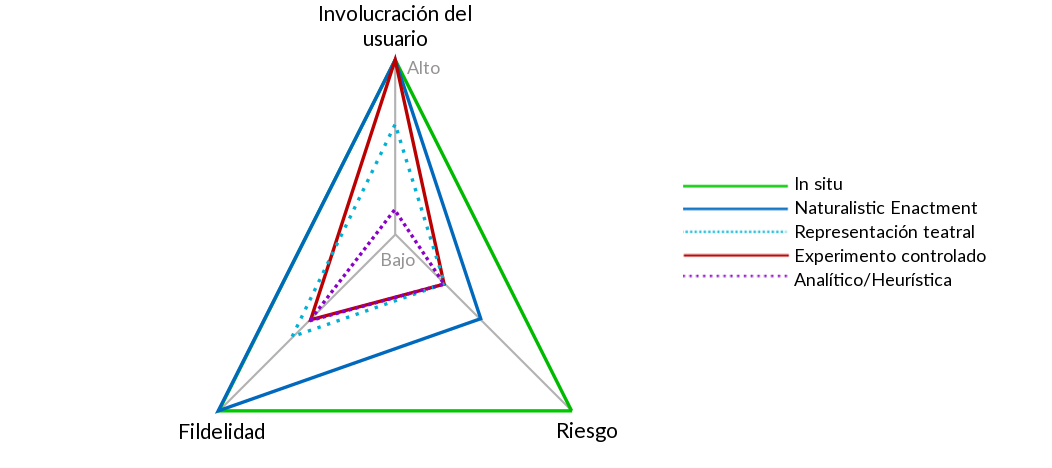
\includegraphics[width=160mm]{./Figures/img_evalmethods}}
        \caption{M\'etodos de evaluaci\'on clasificados de acuerdo a la involucraci\'on del usuario, fidelidad y riesgo}\label{fig:evalmethods}
\end{figure}


Para poder exponer a los sujetos a una situaci\'on de cuidador estresante y realista bajo condiciones controladas, se formul\'o un ejercicio que consisti\'o de una situaci\'on de terapia real con una persona actuando como si tuviera demencia. Un adulto mayor de 75 a\~nos actu\'o como si sufriera de demencia. Se le entren\'o con los comportamientos t\'ipicos de demencia moderada como: murmureo, gritos, vagabundeo, preguntas repetitivas, entre otras. Ella ya estaba familiarazada con estos comportamientos por conocidos que sufrieron de demencia. A los participantes se les dijo que estar\'ian trabajando con una persona que realmente ten\'ia demencia. Tambi\'en, se les ocult\'o la verdadera raz\'on del estudio. En cambio, se les dijo que se les estaba evaluando su rendimiento como cuidadores basados en el entrenamiento inicial que se les di\'o.

Se les pidi\'o firmar un documento de no divulgaci\'on (Ver Ap\'endice~\ref{aped:B} )para evitar que los participantes hablaran entre ellos acerca del experimento, de los comportamientos del adulto mayor o cualquier otra t\'ecnica acerca de como manejar el comportamiento del adulto mayor, durante el tiempo en que el experimento durara.

\subsection{Sujetos}\label{secc:subjects}
Los sujetos fueron reclutados a trav\'es de la lista de correo de CICESE. Se les otorg\'o un premio de compensaci\'on de 100.00 MXN en dinero electr\'onico para el cine. Se les pidi\'o a los participantes asisitr a 3 sesiones (una por cada semana), cada sesi\'on requiri\'o al rededor de 90 minutos de su tiempo. Solo pudieron participar personas que no fueran cuidadores formales, y que no fueran cuidadores en el momento. Se incluyeron a personas que tuvieran experiencia como cuidadores informales. Se obtuvo consentimiento firmado de todos los sujetos (Ver Ap\'endice ~\ref{aped:A} )

Todos los sujetos participaron en una sesi\'on de entrenamiento, en donde se les explic\'o las actividades a realizar en las terapias que hicieron con el adulto mayor.
Participaron 10 estudiantes (5 hombres y 5 Mujeres) con un promedio de 24.5 a\~nos de edad ($\sigma=1.059$). La tabla \ref{table:kysymys} muestra los datos demogr\'aficos de los participantes.
\begin{table}
	\footnotesize
	\centering
	\caption{Participantes en el estudio}
	\label{table:kysymys}
	%\rotatebox{90}{
	\begin{tabular}{m{0.2cm}m{2.5cm}m{2.5cm}m{2.5cm}m{2.5cm}}
		\hline\noalign{\smallskip}
		 & \textbf{Sujeto} & \textbf{G\'enero} & \textbf{Edad} & \textbf{Experiencia de cuidador}
		\\ \noalign{\smallskip}
		\hline
		\noalign{\smallskip}
		&S1& Masculino & 24 & No   \\ 
		&S2& Masculino &  25&  No  \\ 
		&S3& Femenino & 24 & No   \\ 
		&S4& Femenino & 26 & No  \\ 
		&S5& Femenino & 24 & No   \\ 
		&S6& Masculino & 26 &  No  \\ 
		&S7& Masculino & 23 &  No \\ 
		&S8& Masculino & 25 &  Si  \\ 
		&S9& Femenino & 26 & No   \\ 
	  	&S10& Femenino & 24 & Si  \\ 
		\hline
	\end{tabular}
	%}
\end{table}
\section{Procedimiento}\label{secc:methods}
\subsection{Entrenamiento}\label{secc:training}
Todos los sujetos participaron en una sesi\'on de entrenamiento para familiarizarse con las terapias cognitivas que har\'ian con el adulto mayor. La sesi\'on de entrenamiento dur\'o aproximadamente 90 minutos. Todos los participantes practicaron las terapias y tuvieraon oportunidad de hacer preguntas. No se les di\'o ninguna estrategia de afrontamiento acerca de como lidiar con los coportamientos del adulto mayor. Se les dijo a los participantes que el adulto mayor ten\'ia declive cognitivo ligero y que podr\'ia mostrar algunos problemas de comportamiento como olvidar instrucciones recientes, apat\'ia y renuencia de completar las tareas, entre otras. Se les dijo que las tareas no ten\'ian que ser completadas si el adulto mayor no estaba cooperando, pero que deber\'ian intentar completar la terap\'ia en lo posible.

\subsection{Tareas de terapias}\label{secc:therapytasks}
Antes de iniciar la tarea, equipamos a los participantes con una banda de pecho Zephyr Hxm para monitorizar su ritmo card\'iaco, una pulsera Empatica E3 para obtener GSR y temperatura corporal y una banda cerebral Muse para obtener datos de EEG. Todas las sesiones fueron videograbadas para analizarlas posteriormente.

Durante cinco minutos, ya equipados con los dispositivos, se les pidi\'o a los sujetos relajarase concentrandose en su respiraci\'on con los ojos cerrados para obtener una l\'inea base de datos fisiol\'ogicos. S\'olo una persona necesit\'o mas de 5 minutos.

Se les pidi\'o a los participantes que guiaran al adulto mayour a trav\'es de una sesi\'on de terapia que involucr\'o una de las 7 posibles tareas que fueron explicadas durante la sesi\'on de entrenamiento. La tabla ~\ref{table:therapies} presenta las tareas realizadas por cada participante en las tres sesiones del estudio.

\begin{table}[h]
	\footnotesize
	\centering
	\caption{Terapias realizadas con el adulto mayor por cada participante.}
	\label{table:therapies}
	%\rotatebox{90}{
	\begin{tabular}{m{0.2cm}m{2.5cm}m{2.5cm}m{2.5cm}m{2.5cm}}
		\hline\noalign{\smallskip}
	&\textbf{Participante}&  \textbf{Terapia 1}& \textbf{Terapia 2}   & \textbf{Terapia 3}  \\ \hline
		\\ \noalign{\smallskip}
		&S1&  Atado de agujetas& Memorama & Clasificaci\'on de im\'agenes   \\ 
  &S2&  Clasificaci\'on de im\'agenes& Atado de agujetas & Cruzigrama   \\ 
  &S3&  Formaci\'on de palabras& Cruzigrama & Memorama    \\ 
  &S4&  Atado de agujetas& Clasificaci\'on de im\'agenes & Memorama   \\ 
  & S5&  Clasificaci\'on de im\'agenes&  Atado de agujetas & Cruzigrama   \\ 
  &S6&  Separaci\'on de objetos& Memorama & Atado de agujetas   \\ 
  &S7&  Separaci\'on de objetos & Atado de agujetas & Cruzigrama   \\ 
  &S8&  Cruzigrama& Atado de agujetas & Clasificaci\'on de im\'agenes   \\ 
  &S9&  Formaci\'on de palabras& Clasificaci\'on de im\'agenes & Memorama   \\ 
  &S10&  Memorama& Formaci\'on de palabras & Atado de agujetas   \\ 
		\hline
	\end{tabular}
	%}
\end{table}
%\begin{itemize}
%	\item Atado de agujetas.
%%	\item Separaci\'on de objetos.
%	\item Memorama.
%	\item Clasificaci\'on de im\'agenes.
%	\item Formaci\'on de palabras with syllables.
%	\item Sentences with words.
%	\item Formaci\'on de palabras.
%	\item Cruzigrama.
%\end{itemize}

Toda la intervenci\'on dur\'o 15 d\'ias, cada prueba de los participantes dur\'o al rededor de 30 minutos. Cada d\'ia dos participantes asistieron al sitio.

Cada participante asisiti\'o a tres sesiones. Por cada sesi\'on, una o dos tareas fueron hechas, con varias iteraciones en cada tarea. Ninguna de las terapias fueron repetidas por los particpantes. Adem\'as, ninguno de los participantes asisti\'o con el mismo compa\~nero mas de una vez.

Se dividi\'o el experimento en tres semanas. Cada sujeto particip\'o una vez cada semana. Se entren\'o al adulto mayor para actuar con diferentes niveles de ansiedad. En la primer semana, ella actu\'o en niveles de 0 a 2 (Ver tabla ~\ref{table:anxilevels}). En la segunda y tercer semana, actu\'o niveles de 0 a 3. En la \'ultima, se les ense\~n\'o a los participantes a usar estrategias de afrontamiento.
\section{Configuraci\'on}\label{secc:setup}
	Se acondicion\'o un cuarto dentro de una casa real para hacerlo parecer como si fuera la sala de una persona con demencia. La utiler\'ia incluy\'o: Muebles viejos, baja iluminaci\'on, fotograf\'ias viejas, pistas de papel sobre el lavamanos, entre otras. Una mesa de madera fue usada para instalar el equipo: una Macbook, una videoc\'amara, y un tel\'efono inteligente para monitorizar el experimento.
\begin{figure}[h]
        \centering
        \subfigure[]{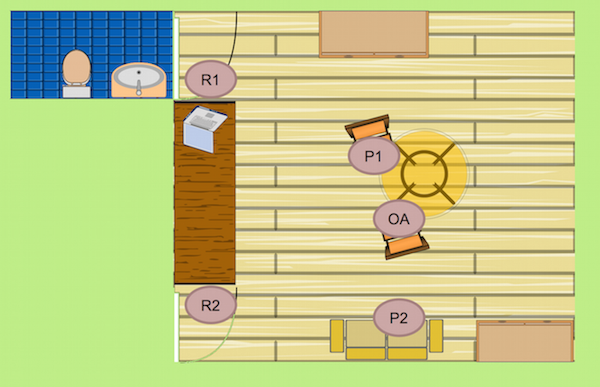
\includegraphics[width=160mm,height=80mm]{./Figures/img_exp_setup}}
        \caption{Escenario experimental. Las actividades fueron realizadas sobre una mesa, con la persona con demencia (OA) y el participante (P1) sentados frente a frente. El segundo participante (P2) observaba sobre el sof\'a, mientras que dos investigadores (R1,R2) monitoreaban la sesi\'on desde una mesa cercana.} \label{fig:img_exp_setup}
\end{figure}

Dos investigadores permanecieron parados al lado de la mesa de madera para operar el equipo y tomar notas (Ver figura ~\ref{fig:img_exp_setup} ). La persona que actuaba como si tuviera demencia y el cuidador permanecieron sentados frente a frente en una mesa circular. Se les pidi\'o a los participantes usar el cuarto de ba\~no para vestir la banda Zephyr debido a que se pone debajo de la ropa. Un segundo participante se sent\'o sobre el sof\'a y le pedimos que observara la sesi\'on. Este participante tambi\'en fue monitorizado por medio de \'unicamente una pulsera Empatica E3.


\subsection{Obtenci\'on de datos}\label{secc:datagathering}
Se desarrollaron dos aplicaciones separadas para el sensor Empatica E3 y el banda Zephyr HxM. Para el primer dispositivo se desarroll\'o la aplicaci\'on ``Care Me Too'' para android (ver figura ~\ref{fig:caremetoo}) la cual se conecta al dispositivo E3 v\'ia Bluetooth Low Energy (BLE), muestra los datos en tiempo real y los guarda en formato .csv. Esta aplicaci\'on tambi\'en puede ayudar a etiquetar eventos con ayuda del usuario, haciendola \'util para estudios naturalistas.


\begin{figure}[h]
        \centering
        \subfigure[]{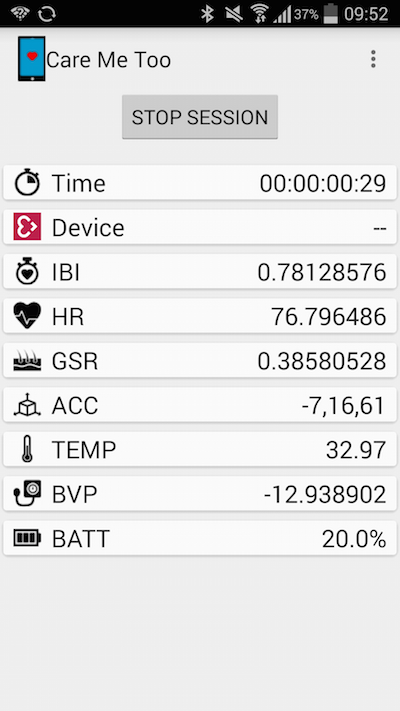
\includegraphics[height=80mm]{./Figures/img_caremetoo}}
        \caption{La aplicaci\'on Care Me Too mostrando se\~nales fisiol\'ogicas siendo grabadas.}\label{fig:caremetoo}
\end{figure}

Para la banda Zephyr HxM se utiliz\'o el programa de l\'inea de comandos ``anxiLogger''\footnote{https://github.com/panzerfausten/anxiLogger} desarrollado para un estudio anterior \citep{Miranda}. El archivo csv de salida fue agregado a los datos de sesi\'on para sincronizar los tiempos a trav\'es de una librer\'ia llamada ``maxiProcesser''\footnote{https://github.com/panzerfausten/maxiProcesser}
\\
Para la banda Muse se us\'o la aplicaci\'on de escritorio ``Muse lab'' Los datos obtenidos en formato .muse fueron exportados a .csv para analizarlos posteriormente.
\\
Se us\'o una laptop Macbook en el sitio para conectar las bandas Muse y Zephyr y un tel\'efono inteligente Samsung Galaxy S4 para colectar datos. Los datos del participante observador fueron obtenidos a trav\'es de una segunda pulsera Empatica E3 en modo de grabaci\'on. Este modo no requiere de una conexi\'on bluetooth.

\section{An\'alisis de los datos}\label{secc:dataanalysis}
Todos los videos de las sesiones fueron analizados para segmentar los eventos de inter\'es. Los eventos eran marcados cuando el adulto mayor actuaba un comportamiento que pudiera inducir ansiedad en el sujeto. Por ejemplo, en un caso el adulto mayor, mientras se encontraba realizando la terapia pregunt\'o al sujeto: \textit{``?` Donde est\'a mi mam\'a?''}. Estos segmentos fueron clasificados en una de los tres posibles niveles que cumplieran con un criterio (ver tabla ~\ref{table:anxilevels}). Luego, se tom\'o una ventana correspondiente a las se\~nales de GSR,HR, temperatura corporal y EEG. Las se\~nales se procesaron individualmente.


\begin{table}
	\footnotesize
	\centering
  	\caption{Criterio de etiquetado de eventos.}
	\label{table:anxilevels}
	\caption{Terapias realizadas con el adulto mayor por cada participante.}
	\label{table:therapies}
	%\rotatebox{90}{
	\begin{tabular}{m{2.5cm}m{5.0cm}m{5.0cm}m{2.5cm}}
		\hline\noalign{\smallskip}

	    \textbf{Nivel} & \textbf{Criterio}                                                                                    & \textbf{Ejemplo de evento}                                                                      \\ \hline
		\\ \noalign{\smallskip}

		    0     & \pbox{12cm}{La PcD est\'a siendo pasiva.,\\La PcD accede a participar.,  \\El participante y la PcD \\est\'an haciendo la tarea} &                   \pbox{12cm}{La PcD est\'a realizando la\\ tarea como se le pidi\'o.}                       \\ 
      1     & \pbox{12cm}{Comportamientos renuentes.,\\Reacio a participar,\\Quejandose acerca de la tarea.}                & \pbox{12cm}{ ``No me gusta este juego.'' \\ ``Esto es muy dif\'icil.'' \\``Hazlo tu.'' }             \\ 
      2     & \pbox{12cm}{Murmureo,\\Hablando cosas sin sentido,  \\Comportamientos impredecibles}                                      & \pbox{5cm}{``?`Donde est\'a mi mam\'a?''\\``Qui\'en eres?''}                                          \\ 
      3     & \pbox{12cm}{Gritos.\\Amenazas al particpante,\\Paranoia,  \\Urgencia de irse.}                          & \pbox{12cm}{``MAM\'A, DONDE EST\'AS!!??''\\``YA QUIERO IRME!''  \\``QUIEN ERES? D\'EJAME IR!'' } \\ 
		\hline
	\end{tabular}
	%}
\end{table}

\subsection{Pre-procesado de GSR}\label{secc:gsrpreprocessing}
Se desarroll\'o una librer\'ia en python para procesar todos los datos fisiol\'ogicos, incluyendo funciones para exportar, extraer caracter\'isticas, sincronizaci\'on de tiempos, y graficado de datos de ansiedad de todos los dispositivos. La librer\'ia tambi\'en puede graficar atributos de la se\~nal GSR (picos, tiempos de recuperaci\'on medios, amplitudes, etc.) en formato .csv y .json.

Se inici\'o remuestreando los datos de GSR de 4.0 Hz a 1.0 Hz calculando el valor promedio de todos los datos que cayeran en una ventana deslizante de 1 segundo. Esto se hizo debido a que se esperaba que los lapsos de ansiedad duraran segundos. Luego, se aplic\'o un filtro gausiano para suavizar la se\~nal y el ruido. Finalmente, se us\'o un m\'etodo de la librer\'ia scipy de python para detectar picos y filtar todos los picos mas grandes que un umbral ($t \geqslant 0.04$ para datos no normalizados). Tambi\'en se calcul\'o el ``Tiempo de media recuperaci\'on'' de la se\~nal. Esto es, el punto donde la se\~nal decae al valor exacto de la mitad del pico.

\subsection{Pre-procesamiento de HR e IBI}\label{secc:hribipreprocessing}
No fue necesario remuestrear los datos de HR e IBI debido a la naturaleza de la se\~nal. El sensor solo reporta datos cuando ocurre un latido del coraz\'on. Sin embargo, se agrup\'o en ventanas de segundos para compararlo con el resto de las se\~nales. El ruido de los datos fu\'e muy bajo y no requiri\'o pre-procesamiento adicional.

\subsection{Procesamiento de video}\label{secc:videoprocesing}
Todos los videos fueron transcritos utilizando el programa F5 transkript para Mac OS X. Luego, se generaron subt\'itulos tomando los tiempos de la transcripci\'on con una herramienta hecha en python y exportados a formato .srt para analizarlos f\'acilmente.
\subsection{Segmentaci\'on de los datos}\label{secc:datasegmentation}
Las transcripciones fueron luego usadas para segmentar los eventos acorde a la tabla ~\ref{table:anxilevels}.
Para obtener ``ground truth'', dos investigadores codificaron las sesiones en vivo, tomando nota del tiempo, nivel de ansiedad percibida, y una descripci\'on del evento. Esta descripci\'on fue escrita en base a lo que el participante y/o la persona con demencia dijo o hizo en el momento. Luego se codificaron los videos vi\'endolos y anotando los tiempos y el nivel de ansiedad percivida. Esta codificaci\'on fue hecha por dos personas mirando todos los videos cada una. Los participantes tambi\'en ten\'ian un formulario en papel para indicar su nivel de ansiedad mientras desarrollaban la tarea. Sin embargo, algunos de ellos encontraron dif\'icil reportarlo, principalmente porque estaban muy ocupados con la tarea.


Una vez etiquetados los segmentos con el nivel percivido de ansiedad. La figura ~\ref{fig:imgsegment} ejemplifica un segmento extra\'ido. En el siguiente cap\'itulo se explica como se clasificaron los datos y los resultados de la detecci\'on.

\begin{figure}[h]
        \centering
        \subfigure[]{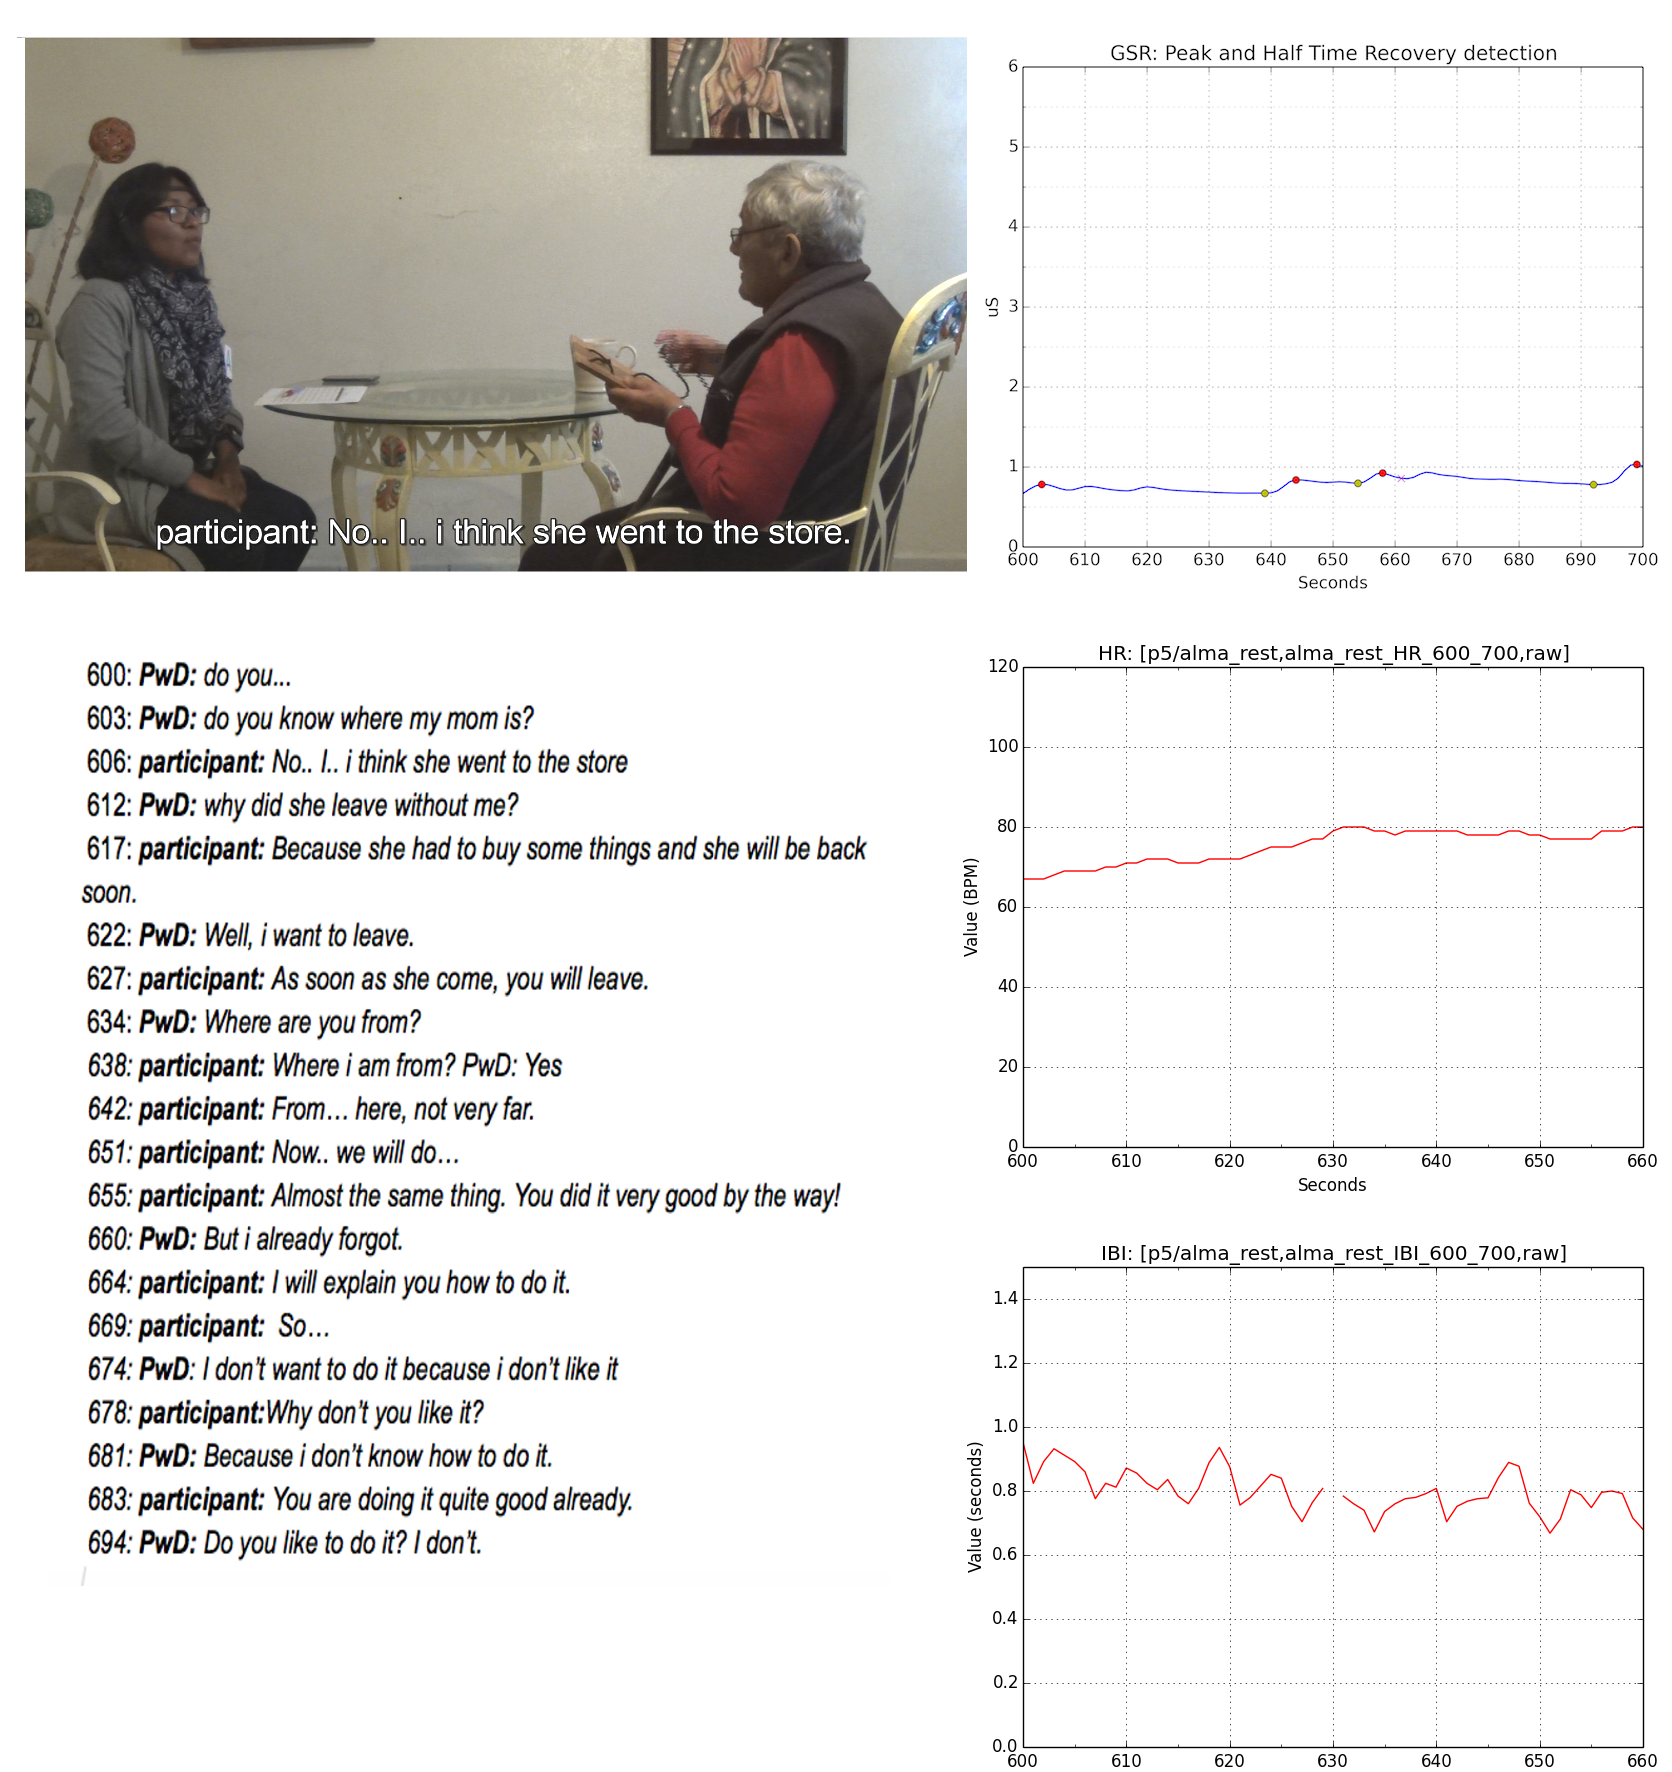
\includegraphics[height=18cm,keepaspectratio]{./Figures/img_segment.png}}
        \caption{Transcripci\'on y se\~nales GSR, HR, e IBI correspondientes a una situaci\'on estresante}\label{fig:imgsegment}
\end{figure}
\newpage
%%=====================================================

